\documentclass[journal,12pt,twocolumn]{IEEEtran}
\usepackage{setspace}
\usepackage{gensymb}
\singlespacing
\usepackage[cmex10]{amsmath}
\usepackage{amsthm}
\usepackage{mathrsfs}
\usepackage{txfonts}
\usepackage{stfloats}
\usepackage{bm}
\usepackage{cite}
\usepackage{cases}
\usepackage{subfig}
\usepackage{longtable}
\usepackage{multirow}
\usepackage{enumitem}
\usepackage{mathtools}
\usepackage{tikz}
\usepackage{circuitikz}
\usepackage{verbatim}
\usepackage[breaklinks=true]{hyperref}
\usepackage{tkz-euclide} % loads  TikZ and tkz-base
\usepackage{listings}
\usepackage{color}    
\usepackage{array}    
\usepackage{longtable}
\usepackage{calc}     
\usepackage{multirow} 
\usepackage{hhline}   
\usepackage{ifthen}   
\usepackage{lscape}     
\usepackage{chngcntr}
\DeclareMathOperator*{\Res}{Res}
\renewcommand\thesection{\arabic{section}}
\renewcommand\thesubsection{\thesection.\arabic{subsection}}
\renewcommand\thesubsubsection{\thesubsection.\arabic{subsubsection}}

\renewcommand\thesectiondis{\arabic{section}}
\renewcommand\thesubsectiondis{\thesectiondis.\arabic{subsection}}
\renewcommand\thesubsubsectiondis{\thesubsectiondis.\arabic{subsubsection}}
\renewcommand\thetable{\arabic{table}}
% correct bad hyphenation here
\hyphenation{op-tical net-works semi-conduc-tor}
\def\inputGnumericTable{}                                 %%

\lstset{
%language=C,
frame=single, 
breaklines=true,
columns=fullflexible,
literate=
{-}{$\rightarrow{}$}{1},
}
%\lstset{
%language=tex,
%frame=single, 
%breaklines=true
%}

\DeclareMathOperator*{\argmax}{arg\,max}
\DeclareMathOperator*{\argmin}{arg\,min}
\begin{document}
\newtheorem{theorem}{Theorem}[section]
\newtheorem{problem}{Problem}
\newtheorem{proposition}{Proposition}[section]
\newtheorem{lemma}{Lemma}[section]
\newtheorem{corollary}[theorem]{Corollary}
\newtheorem{example}{Example}[section]
\newtheorem{definition}[problem]{Definition}
\newcommand{\BEQA}{\begin{eqnarray}}
\newcommand{\EEQA}{\end{eqnarray}}
\newcommand{\define}{\stackrel{\triangle}{=}}
\bibliographystyle{IEEEtran}
\providecommand{\mbf}{\mathbf}
\providecommand{\pr}[1]{\ensuremath{\Pr\left(#1\right)}}
\providecommand{\qfunc}[1]{\ensuremath{Q\left(#1\right)}}
\providecommand{\sbrak}[1]{\ensuremath{{}\left[#1\right]}}
\providecommand{\lsbrak}[1]{\ensuremath{{}\left[#1\right.}}
\providecommand{\rsbrak}[1]{\ensuremath{{}\left.#1\right]}}
\providecommand{\brak}[1]{\ensuremath{\left(#1\right)}}
\providecommand{\lbrak}[1]{\ensuremath{\left(#1\right.}}
\providecommand{\rbrak}[1]{\ensuremath{\left.#1\right)}}
\providecommand{\cbrak}[1]{\ensuremath{\left\{#1\right\}}}
\providecommand{\lcbrak}[1]{\ensuremath{\left\{#1\right.}}
\providecommand{\rcbrak}[1]{\ensuremath{\left.#1\right\}}}
\providecommand{\floor}[1]{\ensuremath{\lfloor #1 \rfloor}}
\providecommand{\lfloor}[1]{\ensuremath{\lfloor #1 \right.}}
\providecommand{\rfloor}[1]{\ensuremath{\left.#1 \rfloor}}
\theoremstyle{remark}
\newtheorem{rem}{Remark}
\newcommand{\sgn}{\mathop{\mathrm{sgn}}}
\newcommand{\re}{\mathop{\mathrm{Re}}}
\providecommand{\abs}[1]{\left\vert#1\right\vert}
\providecommand{\res}[1]{\Res\displaylimits_{#1}} 
\providecommand{\norm}[1]{\left\lVert#1\right\rVert}
\providecommand{\mtx}[1]{\mathbf{#1}}
\providecommand{\mean}[1]{E\left[ #1 \right]}   
\providecommand{\fourier}{\overset{\mathcal{F}}{ \rightleftharpoons}}
\providecommand{\system}[1]{\overset{\mathcal{#1}}{ \longleftrightarrow}}
\newcommand{\solution}{\noindent \textbf{Solution: }}
\newcommand{\cosec}{\,\text{cosec}\,}
\providecommand{\dec}[2]{\ensuremath{\overset{#1}{\underset{#2}{\gtrless}}}}
\newcommand{\myvec}[1]{\ensuremath{\begin{pmatrix}#1\end{pmatrix}}}
\newcommand{\mydet}[1]{\ensuremath{\begin{vmatrix}#1\end{vmatrix}}}
\renewcommand{\vec}[1]{\boldsymbol{\mathbf{#1}}}
\def\putbox#1#2#3{\makebox[0in][l]{\makebox[#1][l]{}\raisebox{\baselineskip}[0in][0in]{\raisebox{#2}[0in][0in]{#3}}}}
     \def\rightbox#1{\makebox[0in][r]{#1}}
     \def\centbox#1{\makebox[0in]{#1}}
     \def\topbox#1{\raisebox{-\baselineskip}[0in][0in]{#1}}
     \def\midbox#1{\raisebox{-0.5\baselineskip}[0in][0in]{#1}}

\vspace{3cm}
\title{Advanced DSP (EE5900)\\Homework Assignment 3}
\author{Gautam Singh\\CS21BTECH11018}
\maketitle
\bigskip

\begin{enumerate}[label=\theenumi.]
    \item 
    \begin{enumerate}
        \item Using the inverse Fourier transform,
        \begin{align}
            x_a\brak{t} &= \frac{1}{2\pi}\int_{-\infty}^{\infty}X_a\brak{j\Omega}e^{j\Omega{}t}d\Omega, \\
            x\brak{n} &= \frac{1}{2\pi}\int_{-\pi}^{\pi}X\brak{e^{j\omega}}e^{j\omega{}n}d\omega.
            \label{eq:x-ift}
        \end{align}
        However, we also know that
        \begin{align}
            x\brak{n} &= x_a\brak{nT} = x_a\brak{t}\rvert_{t=nT} \\
            &= \frac{1}{2\pi}\int_{-\infty}^{\infty}X_a\brak{j\Omega}e^{j\Omega{}nT}d\Omega \\
            &= \frac{1}{2\pi}\sum_{r=-\infty}^{\infty}\int_{\brak{2r-1}\frac{\pi}{T}}^{\brak{2r+1}\frac{\pi}{T}}X_a\brak{j\Omega}e^{j\Omega{}nT}d\Omega.
            \label{eq:x-n-sub}
        \end{align}
        Making a change of variables for each term in the summation, \(\Omega
        \rightarrow \Omega + \frac{2\pi{}r}{T}\),
        \begin{multline}
            x\brak{n} = \frac{1}{2\pi}\sum_{r=-\infty}^{\infty}\int_{-\frac{\pi}{T}}^{\frac{\pi}{T}}X_a\brak{j\Omega+j\frac{2\pi{}r}{T}} \\
            e^{j\Omega{}nT}e^{j2\pi{}rn}d\Omega.
            \label{eq:x-n-sum}
        \end{multline}
        Interchanging the order of summation and integration, and noting that
        \(e^{j2\pi{}rn} = 1\ \forall\ n\in\mathbb{Z},\ r\in\mathbb{Z}\),
        \begin{multline}
            x\brak{n} = \frac{1}{2\pi}\int_{-\frac{\pi}{T}}^{\frac{\pi}{T}}\sbrak{\sum_{r=-\infty}^{\infty}X_a\brak{j\Omega+j\frac{2\pi{}r}{T}}} \\
            e^{j\Omega{}nT}d\Omega.
        \end{multline}
        Making the substitution \(\Omega = \frac{\omega}{T}\),
        \begin{multline}
            x\brak{n} = \frac{1}{2\pi}\int_{-\pi}^{\pi}\sbrak{\frac{1}{T}\sum_{r=-\infty}^{\infty}X_a\brak{j\frac{\omega}{T}+j\frac{2\pi{}r}{T}}} \\
            e^{j\omega{}n}d\omega.
            \label{eq:x-n-a}
        \end{multline}
        Comparing \eqref{eq:x-ift} with \eqref{eq:x-n-a}, we obtain
        \begin{equation}
            X\brak{e^{j\omega}} = \frac{1}{T}\sum_{r=-\infty}^{\infty}X_a\brak{\frac{j\omega}{T} + j\frac{2\pi{}r}{T}}.
            \label{eq:omega-rel}
        \end{equation}
        where \(\Omega = \frac{\omega}{T}\).

        \item Consider a signal \(x_a\brak{t} = A\cos\brak{2\pi{}Ft + \phi}\)
        sampled every \(T\) seconds. The sampling frequency \(F_s\) is given by
        \begin{equation}
            F_s = \frac{1}{T}
            \label{eq:F-s-t}
        \end{equation}
        and the sampled discrete time signal is
        \begin{align}
            x\brak{n} &= x_a\brak{nT} \\
            &= A\cos\brak{2n\pi{}FT + \phi} \\
            &= A\cos\brak{2n\pi{}\frac{F}{F_s} + \phi}.
            \label{eq:norm-f}
        \end{align}
        From \eqref{eq:norm-f}, we see that the normalized digital frequency is
        given by
        \begin{equation}
            f \define \frac{F}{F_s} = FT.
            \label{eq:rel-f-F-T}
        \end{equation}

        \item The ranges are given in \autoref{tab:range}.
        \begin{table}[!ht]
            \centering
            \begin{tabular}{|c|c|}
                \hline
                \textbf{Quantity} & \textbf{Range} \\
                \hline
                \(\omega\) & \(\rsbrak{\lbrak{-\pi,\pi}}\) \\
                \hline
                \(\Omega\) & \(\brak{-\infty,\infty}\) \\
                \hline
                \(f\) & \(\rsbrak{\lbrak{-\frac{1}{2},\frac{1}{2}}}\) \\
                \hline
                \(F\) & \(\brak{-\infty,\infty}\) \\
                \hline
                \(F_s\) & \(\brak{-\infty,\infty}\) \\
                \hline
                \(T\) & \(\brak{-\infty,\infty}\) \\
                \hline
            \end{tabular}
            \caption{Range of various quantities.}
            \label{tab:range}
        \end{table}

        \item By sampling theorem, we know that all analog frequencies of the
        input signal are mapped to the range \(\lbrak{\rsbrak{-\frac{F_s}{2},\frac{F_s}{2}}}\).
        Therefore, the range of digital frequency that can be obtained,
        \begin{equation}
            f = \frac{F}{F_s} \in \lbrak{\rsbrak{-\frac{1}{2}, \frac{1}{2}}}.
            \label{eq:f-range}
        \end{equation}
        Hence, the maximum obtainable digital frequency is \(\frac{1}{2}\)
        at \(F = \brak{2n+1}\frac{F_s}{2},\ n \in \mathbb{Z}\).

        \item We know that
        \begin{align}
            f = \frac{F}{F_s} \le \frac{1}{2} \\
            \implies F \le \frac{F_s}{2}.
        \end{align}
        Thus, for a given \(f\) and \(F_s\), the maximum analog frequency is
        \(\frac{F_s}{2}\).

        \item The units are given in \autoref{tab:unit}. Where no units are
        mentioned, it means that the quantity is dimensionless.
        \begin{table}[!ht]
            \centering
            \begin{tabular}{|c|c|}
                \hline
                \textbf{Quantity} & \textbf{Units} \\
                \hline
                \(\omega\) & \\
                \hline
                \(\Omega\) & rad s\textsuperscript{-1} \\
                \hline
                \(f\) & \\
                \hline
                \(F\) & Hz \\
                \hline
                \(F_s\) & Hz \\
                \hline
                \(T\) & s \\
                \hline
            \end{tabular}
            \caption{Units of various quantities.}
            \label{tab:unit}
        \end{table}
    \end{enumerate}

    \item The given input signal is
    \begin{equation}
        x_a\brak{t} = 3\cos\brak{100\pi{}t} + 2\sin\brak{250\pi{}t}
        \label{eq:x-in}
    \end{equation}
    and the frequency response is
    \begin{multline}
        X_a\brak{j\Omega} = 3\pi\brak{\delta\brak{\Omega-100\pi} + \delta\brak{\Omega+100\pi}} \\
        - 2j\pi\brak{\delta\brak{\Omega-250\pi} - \delta\brak{\Omega+250\pi}}
    \end{multline}
    as shown in \autoref{fig:inp-spectrum}.

    \begin{figure}[!ht]
        \centering
        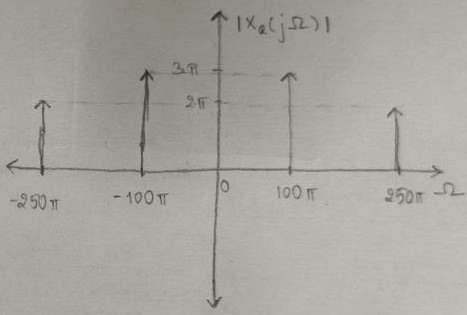
\includegraphics[width=\columnwidth]{figs/inp-spectrum.jpg}
        \caption{Spectrum of input signal.}
        \label{fig:inp-spectrum}
    \end{figure}

    After the ADC stage, the output waveform is obtained by setting
    \(t = nT_1\). Thus,
    \begin{align}
        x\brak{n} &= x_a\brak{nT_1} \\
                  &= 3\cos\brak{\frac{n\pi}{2}} + 2\sin\brak{\frac{5n\pi}{4}} \\
                  &= 3\cos\brak{\frac{n\pi}{2}} + 2\sin\brak{\frac{-3n\pi}{4}}
                  \label{eq:x-adc}
    \end{align}
    and the frequency response is (for \(-\pi < \omega \le \pi\))
    \begin{multline}
        X\brak{\omega} = 3\pi\brak{\delta\brak{\omega-\frac{\pi}{2}} + \delta\brak{\omega+\frac{\pi}{2}}} \\
        + \frac{2\pi}{j}\brak{\delta\brak{\omega+\frac{3\pi}{4}} - \delta\brak{\omega-\frac{3\pi}{4}}}
        \label{eq:dtft-xn}
    \end{multline}
    which is periodic with period \(2\pi\). The spectral content of the
    principal range is shown in \autoref{fig:adc-spectrum}.
    
    \begin{figure}[!ht]
        \centering
        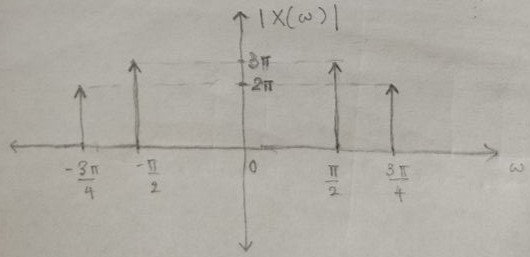
\includegraphics[width=\columnwidth]{figs/adc-spectrum.jpg}
        \caption{Spectrum after ADC stage (\(-\pi < \omega \le \pi\)).}
        \label{fig:adc-spectrum}
    \end{figure}

    At the DAC stage, we upsample the input digital signal by a factor of
    \(\frac{T_1}{T_2} = 5\), by padding 4 zeros between each sample. Denote the
    zero-padded signal by \(\tilde{x}\brak{k}\). Then,
    \begin{equation}
        \tilde{x}\brak{k} =
        \begin{cases}
            x\brak{m} & k = 5m,\ m \in \mathbb{Z} \\
            0 & \text{ otherwise}
        \end{cases}.
        \label{eq:x-tilde}
    \end{equation}
    The output waveform after the DAC stage will be
    \begin{equation}
        \tilde{x}\brak{t} =
        \begin{cases}
            x\brak{m} & 5mT_2 \le t < \brak{5m+1}T_2 \\
            0 & \text{otherwise},
        \end{cases}
    \end{equation}
    and the corresponding frequency response is, noting that \(T_1 = 5T_2\),
    \begin{align}
        \tilde{X}\brak{j\Omega} &= \sum_{m=-\infty}^{\infty}\int_{5mT_2}^{\brak{5m+1}T_2}x\brak{m}e^{-j\Omega{}t}dt \\
        &= \sum_{m=-\infty}^{\infty}\int_{mT_1}^{mT_1+T_2}x\brak{m}e^{-j\Omega{}t}dt \\
        &= \frac{1-e^{-j\Omega{}T_2}}{j\Omega}\sum_{m=-\infty}^{\infty}x\brak{m}e^{-j\brak{\Omega{}T_1}m} \\
        &= \frac{1-e^{-j\Omega{}T_2}}{j\Omega}X\brak{\Omega{}T_1}
        \label{eq:freq-resp-dac}
    \end{align}
    as shown in \autoref{fig:dac-spectrum}.

    \begin{figure}[!ht]
        \centering
        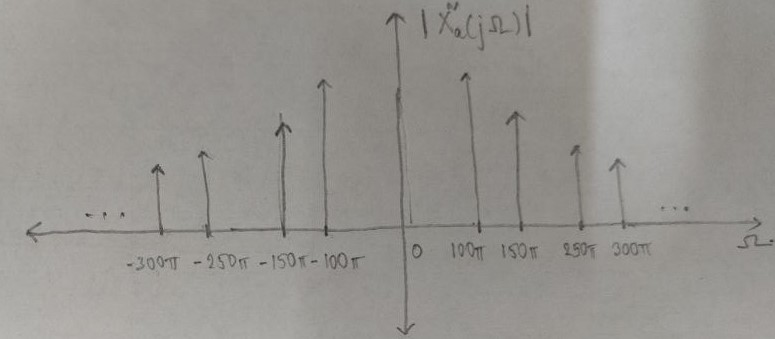
\includegraphics[width=\columnwidth]{figs/dac-spectrum.jpg}
        \caption{Spectrum after upsampling and DAC stage.}
        \label{fig:dac-spectrum}
    \end{figure}

    After the filter stage, from \eqref{eq:x-tilde} and \eqref{eq:x-adc},
    \begin{align}
        Y_{a}\brak{t} &= \sum_{k=-\infty}^{\infty}\tilde{x}\brak{k}h\brak{t-kT_2} \\
                       &= \sum_{r=0}^{4}\sum_{m=-\infty}^{\infty}\tilde{x}\brak{5m+r}h\brak{t-\brak{5m+r}T_2} \\
                       &= \sum_{m=-\infty}^{\infty}x\brak{m}h\brak{t-5mT_2} \\
                       &= \sum_{m=-\infty}^{\infty}x\brak{m}h\brak{t-mT_1} \\
                    \begin{split}
                       = \sum_{m=-\infty}^{\infty}\brak{3\cos\brak{\frac{m\pi}{2}} + 2\sin\brak{\frac{-3m\pi}{4}}}\\
                       h\brak{t-mT_1}
                    \end{split} \\
                       &= 3\cos\brak{100\pi{}t} + 2\sin\brak{-150\pi{}t}.
                       \label{eq:Y-ob}
    \end{align}
    and the corresponding frequency response is
    \begin{multline}
        Y_a\brak{j\Omega} = 3\pi\brak{\delta\brak{\Omega-100\pi} + \delta\brak{\Omega+100\pi}} \\
        - 2j\pi\brak{\delta\brak{\Omega+150\pi} - \delta\brak{\Omega-150\pi}}
    \end{multline}
    as shown in \autoref{fig:filt-spectrum}.

    \begin{figure}[!ht]
        \centering
        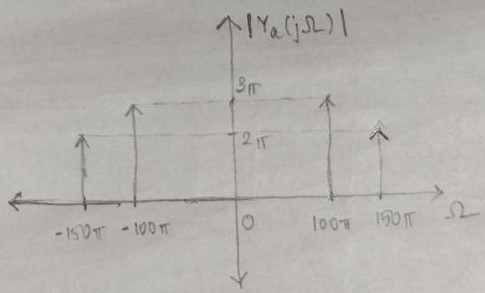
\includegraphics[width=\columnwidth]{figs/filt-spectrum.jpg}
        \caption{Spectrum after the filter stage.}
        \label{fig:filt-spectrum}
    \end{figure}

    Notice that \eqref{eq:Y-ob} and \eqref{eq:x-in} are not equal. This is
    because the ADC undersampled the signal, leading to \emph{aliasing}
    when upsampled by the DAC and filtered.

    \item For a discrete time signal with input range \(A\) and resolution
    \(\Delta\), the number of bits required, \(N\), is given by
    \begin{equation}
        2^N = \left\lceil\frac{A}{\Delta}\right\rceil + 1
        \label{eq:2-N-quant}
    \end{equation}
    and so,
    \begin{equation}
        N = \left\lceil\log_2\brak{\left\lceil\frac{A}{\Delta}\right\rceil + 1}\right\rceil.
        \label{eq:N-val}
    \end{equation}
    For both cases, \(A = 6.35-\brak{-6.35} = 13.7\).
    \begin{enumerate}
        \item \(\Delta = 0.1\). Using \eqref{eq:N-val}, \(N = 8\) bits.
        \item \(\Delta = 0.02\). Using \eqref{eq:N-val}, \(N = 10\) bits.
    \end{enumerate}

    \item To check the linearity of a recursive system, we consider two input
    signals \(x_1\brak{n}\), \(x_2\brak{n}\) and their respective outputs
    \(y_1\brak{n}\), \(y_2\brak{n}\). If for all reals \(a_1,\ a_2\), we have
    \begin{equation}
        h\brak{n} \circledast \brak{a_1x_1\brak{n} + a_2x_2\brak{n}} = a_1y\brak{n} + a_2y\brak{n}.
        \label{eq:linearity}
    \end{equation}
    then the given system is linear. For the given case, we have
    \begin{align}
        y_1\brak{n} &= ay_1\brak{n-1} + x_1\brak{n} \label{eq:y1}, \\
        y_2\brak{n} &= ay_2\brak{n-1} + x_2\brak{n} \label{eq:y2},
    \end{align}
    and so,
    \begin{align}
        &a_1y_1\brak{n} + a_2y_2\brak{n} \nonumber \\
        &= a_1\brak{ay_1\brak{n-1} + x_1\brak{n}} \nonumber \\
        &+ a_2\brak{ay_2\brak{n-1} + x_2\brak{n}} \\
        &= a\brak{a_1y_1\brak{n-1} + a_2y_2\brak{n-1}} \nonumber \\
        &+ \brak{a_1x_1\brak{n}+a_2x_2\brak{n}}.
    \end{align}
    This shows that the system is linear. To show that the system is stable,
    we must show that \(\abs{z} = 1\) lies in the region of convergence (ROC)
    of the system function \(H\brak{z}\). However, from the given recurrence,
    \begin{align}
        Y\brak{z} &= az^{-1}Y\brak{z} + X\brak{z}, \\
        H\brak{z} &= \frac{Y\brak{z}}{X\brak{z}} = \frac{1}{1-az^{-1}}.
        \label{eq:H-z}
    \end{align}
    For \eqref{eq:H-z} to converge, the required ROC is
    \begin{equation}
        \abs{az^{-1}} < 1 \implies \abs{z} > \abs{a},
    \end{equation}
    and since the ROC must contain the unit circle, we must have for stability
    \begin{equation}
        \abs{a} < 1.
        \label{eq:cond-a-stable}
    \end{equation}
    The homogeneous equation is
    \begin{equation}
        y\brak{n} - ay\brak{n-1} = 0.
        \label{eq:y-homogeneous}
    \end{equation}
    Setting \(y\brak{n} = \lambda^n\), we get
    \begin{equation}
        \lambda^{n-1}\brak{\lambda-a} = 0.
        \label{eq:lambda-eqn}
    \end{equation}
    Therefore, \(\lambda = a\). Hence, the homogeneous solution is
    \begin{equation}
        y\brak{n} = a^nu\brak{n}.
    \end{equation}
\end{enumerate}

\end{document}
